\documentclass[12pt]{article}   	% use "amsart" instead of "article" for AMSLaTeX format
\usepackage{amssymb}
\usepackage{amsmath}
\usepackage{graphicx}%
\usepackage{amsfonts}%
%\usepackage{float}
\usepackage{natbib}
\usepackage{floatrow}
\bibliographystyle{agsm}
\setcitestyle{authoryear,open={(},close={)},aysep={}}
\usepackage{xr}
\usepackage{hyperref}
\usepackage{subcaption}
\captionsetup[subfigure]{labelformat=empty}
\usepackage{sidecap}

\usepackage{multirow}
\renewcommand{\baselinestretch}{1.0}
\setlength{\oddsidemargin}{0in} \setlength{\textwidth}{6.5in}
%SetFonts
\newcommand{\blam}{ \mbox{\boldmath $ \lambda $} }
\newcommand{\bet}{ \mbox{\boldmath $ \eta $} }
\newcommand{\btau}{ \mbox{\boldmath $ \tau $} }
\newcommand{\bome}{ \mbox{\boldmath $ \omega $} }
\newcommand{\bbet}{ \mbox{\boldmath $ \beta $} }
\newcommand{\bbeta}{ \mbox{\boldmath $ \beta $} }
\newcommand{\balph}{ \mbox{\boldmath $ \alpha $} }
\newcommand{\balpha}{ \mbox{\boldmath $ \alpha $} }
\newcommand{\bphi}{ \mbox{\boldmath $\phi$}}
\newcommand{\bzeta}{ \mbox{\boldmath $\zeta$}}
\newcommand{\bkap}{ \mbox{\boldmath $\kappa$}}
\newcommand{\bkappa}{ \mbox{\boldmath $\kappa$}}
\newcommand{\beps}{ \mbox{\boldmath $\epsilon$}}
\newcommand{\bepsilon}{ \mbox{\boldmath $\epsilon$}}
\newcommand{\bthet}{ \mbox{\boldmath $ \theta $} }
\newcommand{\btheta}{ \mbox{\boldmath $ \theta $} }
\newcommand{\bnu}{ \mbox{\boldmath $\nu$} }
\newcommand{\bmu}{ \mbox{\boldmath $\mu$} }
\newcommand{\bOmega}{ \mbox{\boldmath $\Omega$} }
\newcommand{\bGam}{ \mbox{\boldmath $\Gamma$} }
\newcommand{\bSig}{ \mbox{\boldmath $\Sigma$} }
\newcommand{\bSigma}{ \mbox{\boldmath $\Sigma$} }
\newcommand{\bPhi}{ \mbox{\boldmath $\Phi$} }
\newcommand{\bThet}{ \mbox{\boldmath $\Theta$} }
\newcommand{\bTheta}{ \mbox{\boldmath $\Theta$} }
\newcommand{\bDel}{ \mbox{\boldmath $\Delta$} }
\newcommand{\bDelta}{ \mbox{\boldmath $\Delta$} }
\newcommand{\bnabla}{ \mbox{\boldmath $\nabla$} }
\newcommand{\bLam}{ \mbox{\boldmath $\Lambda$} }
\newcommand{\bLambda}{ \mbox{\boldmath $\Lambda$} }
\newcommand{\bLambdasub}{ \scriptsize{\bLambda}}
\newcommand{\bgam}{ \mbox{\boldmath $\gamma$} }
\newcommand{\bgamma}{ \mbox{\boldmath $\gamma$} }
\newcommand{\brho}{ \mbox{\boldmath $\rho$} }
\newcommand{\bdel}{ \mbox{\boldmath $\delta$} }
\newcommand{\bdelta}{ \mbox{\boldmath $\delta$} }
\newcommand{\bvarphi}{ \mbox{\boldmath $\varphi$} }
\newcommand{\bsigma}{ \mbox{\boldmath $\sigma$} }
\newcommand{\boeta}{ \mbox{\boldmath $\eta$} }
\newcommand{\bpi}{ \mbox{\boldmath $\pi$} }
\newcommand{\bpsi}{ \mbox{\boldmath $\psi$} }
\newcommand{\bzero}{\textbf{0}}
\newcommand{\bone}{\textbf{1}}
\newcommand{\bZ}{\textbf{Z}}
\newcommand{\bz}{\textbf{z}}
\newcommand{\ba}{\textbf{a}}
\newcommand{\bA}{\textbf{A}}
\newcommand{\bb}{\textbf{b}}
\newcommand{\bB}{\textbf{B}}
\newcommand{\bc}{\textbf{c}}
\newcommand{\bC}{\textbf{C}}
\newcommand{\bd}{\textbf{d}}
\newcommand{\bD}{\textbf{D}}
\newcommand{\be}{\textbf{e}}
\newcommand{\bE}{\textbf{E}}
\newcommand{\bbf}{\textbf{f}}
\newcommand{\bF}{\textbf{F}}
\newcommand{\bk}{\textbf{k}}
\newcommand{\bK}{\textbf{K}}
\newcommand{\bh}{\textbf{h}}
\newcommand{\bH}{\textbf{H}}
\newcommand{\bi}{\textbf{i}}
\newcommand{\bI}{\textbf{I}}
\newcommand{\bg}{\textbf{g}}
\newcommand{\bG}{\textbf{G}}
\newcommand{\bJ}{\textbf{J}}
\newcommand{\bL}{\textbf{L}}
\newcommand{\bm}{\textbf{m}}
\newcommand{\bM}{\textbf{M}}
\newcommand{\bn}{\textbf{N}}
\newcommand{\bN}{\textbf{N}}
\newcommand{\bO}{\textbf{O}}
\newcommand{\bp}{\textbf{p}}
\newcommand{\bP}{\textbf{P}}
\newcommand{\bq}{\textbf{q}}
\newcommand{\bQ}{\textbf{Q}}
\newcommand{\bs}{\textbf{s}}
\newcommand{\bS}{\textbf{S}}
\newcommand{\bt}{\textbf{t}}
\newcommand{\bT}{\textbf{T}}
\newcommand{\bu}{\textbf{u}}
\newcommand{\bU}{\textbf{U}}
\newcommand{\bv}{\textbf{v}}
\newcommand{\bV}{\textbf{V}}
\newcommand{\bw}{\textbf{w}}
\newcommand{\bW}{\textbf{W}}
\newcommand{\bx}{\textbf{x}}
\newcommand{\bX}{\textbf{X}}
\newcommand{\by}{\textbf{y}}
\newcommand{\bY}{\textbf{Y}}
\newcommand{\br}{\textbf{r}}
\newcommand{\bR}{\textbf{R}}
\newcommand{\iidsim}{\overset{\text{iid}}{\sim} }
\newcommand{\indsim}{\stackrel{\mbox{\tiny indep}}{\sim}}
\newcommand{\set}{\overset{\text{set}}{=} }

\newcommand{\E}{\mathbb{E}}

\usepackage{xcolor}
\xdefinecolor{custom_red}{rgb}{0.58, 0.32, 0.32} % Marsala
%% SOLUTIONS -- must comment one out
% OFF
%\newcommand{\soln}[2]{\vspace{0cm}}{}
% ON 
\newcommand{\soln}[2]{\textit{\textcolor{custom_red}{#2}}}{}

\usepackage[headheight=65pt,tmargin=65pt,headsep=5pt, margin = 1in]{geometry}

\usepackage{fancyhdr}
\pagestyle{fancy}

\lhead{STAT 201}
\rhead{Solutions}
\chead{\Large{Practice Problems}}
\renewcommand{\headrulewidth}{0.4pt}
\renewcommand{\footrulewidth}{0pt}
\begin{document}

\subsection*{Intro Hypothesis Testing }

\begin{enumerate}
\item
  For each of the research statements below, determine whether it
  represents a null hypothesis claim or an alternative hypothesis claim.

  \begin{enumerate}
  \item
    The number of hours that grade-school children spend doing homework
    predicts their future success on standardized tests. \soln{}{Alternative}
  \item
    King cheetahs on average run the same speed as standard spotted
    cheetahs. \soln{}{Null}
  \item
    For a particular student, the probability of correctly answer a
    5-option multiple choice test is larger than 0.2 (i.e.~better than
    guessing)  \soln{}{Alternative}
  \item
    The probability of getting in a car accident is the same if using a
    cell phone then if not using a cell phone. \soln{}{Null}
  \end{enumerate}
   
  \item
  Write out the null and alternative hypotheses in words and also in
  statistical notation for each of the following situations. When
  writing in statistical notation, be sure to define quantities in
  context.

  \begin{enumerate}
  \item
    New York is known as ``the city that never sleeps''. A random sample
    of 25 New Yorkers were asked how much they sleep they get per night.
    Does these data providing convincing evidence that New Yorkers on
    average sleep less than 8 hours per night?
    
    \soln{}{$H_{0}: \mu = 8$ (On average New Yorkers sleep 8 hours a night) versus $H_{A}: \mu < 8$ (On average New Yorkers sleep less than 8 hours a night), where $\mu$ is the mean hours of sleep New Yorkers receive. }
    
  \item
    A study suggests that 25\% of 25 year-olds have gotten married. You
    believe that this is incorrect and decide to collect your own data
    to conduct a hypothesis test.
    
        \soln{}{$H_{0}: p = 0.25$ (True proportion of 25 year-olds who have gotten married is 25\%) versus $H_{A}: p \neq 0.25$ (True proportion of 25 year-olds who have gotten married is not 25\%) }
        
  \end{enumerate}
\item
  A Survey USA poll conducted in Seattle, WA in May 2021 reports that of
  the 650 respondents (adults living in this area), 159 support
  proposals to defund police departments.

  \begin{enumerate}
  \item
    A journals writing a news story on the poll results wants to use the
    headline: ``More than 1 in 5 adults living in Seattle support
    proposals to defund police departments''. You caution the journalist
    that they should first conduct a hypothesis test to see if the poll
    data provide convincing evidence for this claim. Write the
    hypotheses for this test using proper notation, defining any
    necessary quantities.
    
    \soln{}{$H_{0}: p = 0.20$ versus $H_{A}: p > 0.20$ where $p$ is the true proportion of Seattle adults who support proposals to defund.}
  \item
    Describe in words a simulation scheme that would be appropriate for
    this situation. Also describe how the p-value can be calculated
    using the simulation results.
    
    \soln{}{Example solution: . Take 100 cards, 20
black cards representing those who support proposals to defund police departments
and 80 red cards representing those who do not. Shuffle the cards and draw with
replacement (shuffling each time in between draws to get our ``infinite population") 650 cards representing the 650
respondents to the poll. After each iteration, calculation $\hat{p}_{sim}$, the  proportion of black cards which represents the simulated proportion of adults in favor. The p-value will be the proportion of simulations where $\hat{p}_{sim} \geq 0.245$.}
    
  \item
    The histogram below shows the distribution of 1000 simulated
    proportions under \(H_{0}\). Estimate the p-value using the plot and
    use it to evaluate your hypotheses (i.e.~make a conclusion). Assume
    a significance level of 0.05.

    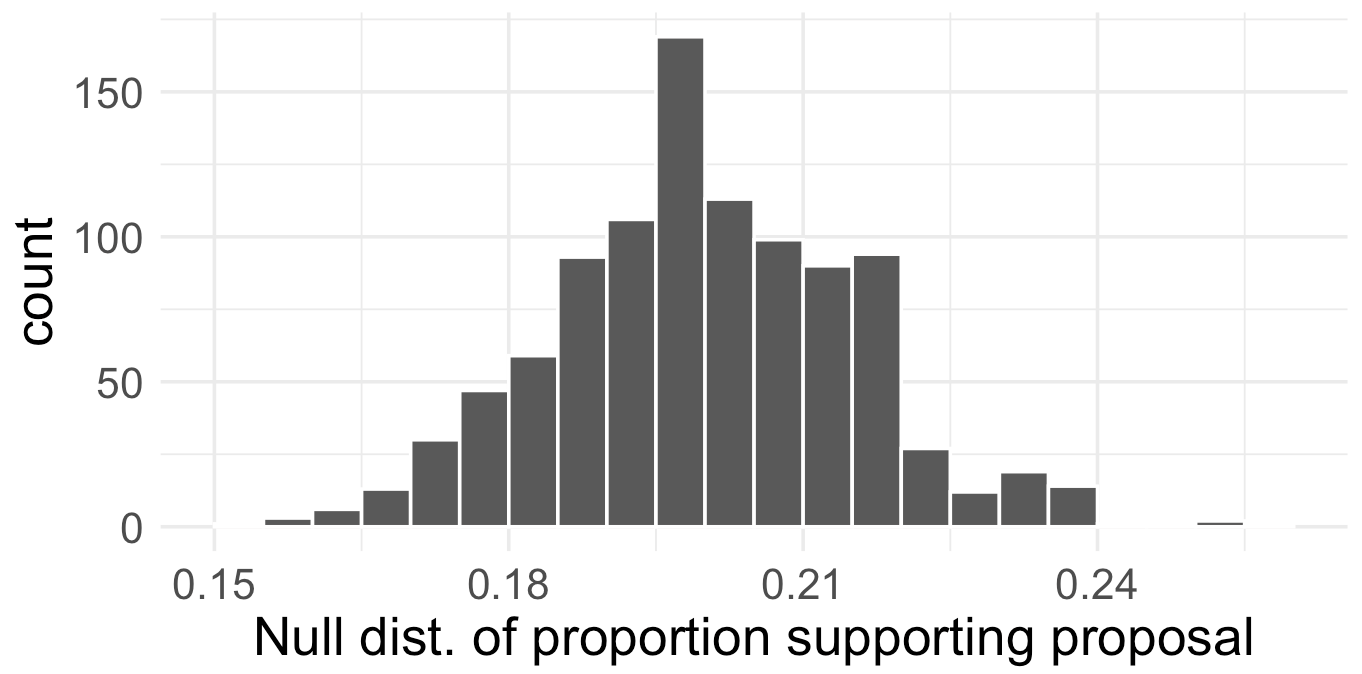
\includegraphics[scale = 0.5]{images/13-defund.png}
    
    \soln{}{There is only one simulated proportion that is at least 0.245, therefore the approximate p-value is 0.001. Since $0.001 < 0.05$, reject $H_{0}$. The data provide convincing evidence that the proportion of Seattle adults who support proposals to
defund police departments is greater than 0.20.}
    
  \end{enumerate}
  
  \item
  A study conducted in 2020 found that the U.S. adjusted divorce rate
  was 14 per 1000 married women. Joe is suspicious and disagrees with
  the stated divorce rate. Joe somehow collected data from 323 married
  or previously-married women, and asked them if they had a divorce in
  2020. 55 of the women responded that they indeed had a divorce in
  2020.

  \begin{enumerate}
  \item
    Write out the hypotheses corresponding to this scenario.
    
    \soln{}{$H_{0}: p = 0.14$ versus $H_{A}: p \neq 0.14$ where $p$ is the true divorce rate among married women.}
    
      \item
    Describe in words a simulation scheme that would be appropriate for
    this situation. Also describe how the p-value can be calculated
    using the simulation results.
    
    \soln{}{Similar to previous problem.}
    
  \item
    The histogram below shows the distribution of 100 simulated
    proportions under \(H_{0}\). Estimate the p-value using the plot and
    use it to evaluate Joe's hypotheses (i.e. make a conclusion). Assume
    a significance level of 0.05.

    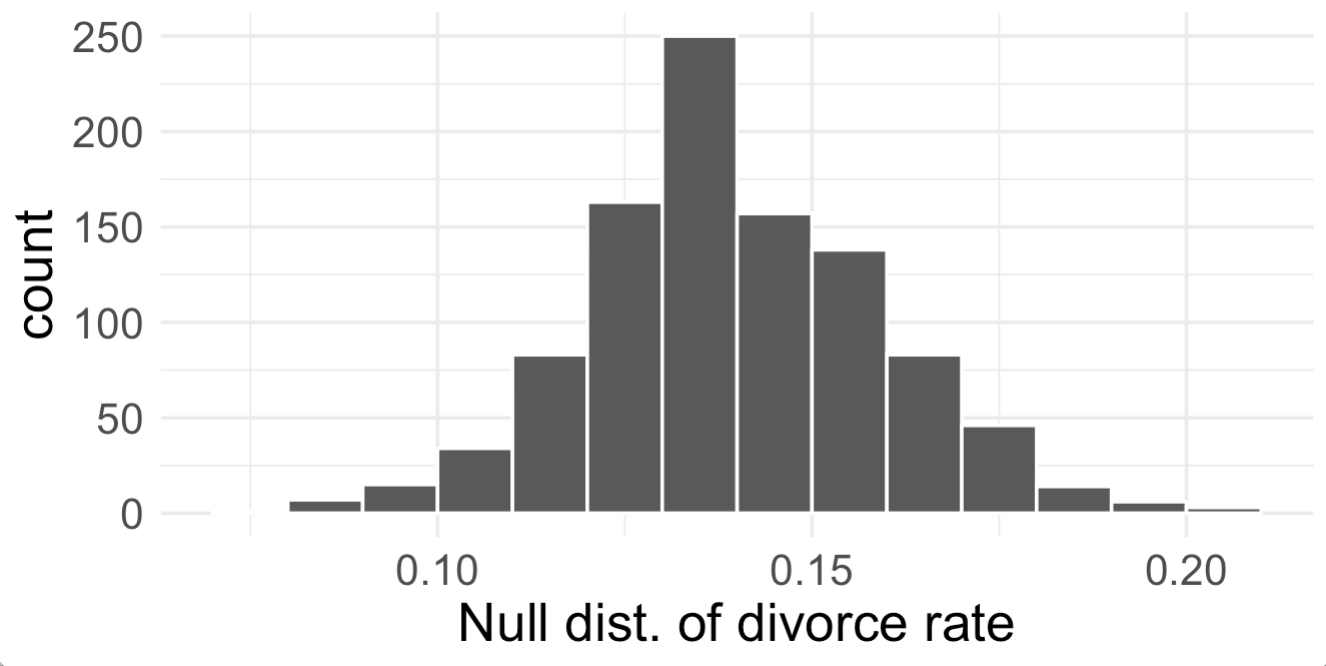
\includegraphics[scale = 0.5]{images/13-divorce.png}
    
    \soln{}{The observed proportion was $\hat{p}_{obs}  = 55/323 = 0.17$. Since the alternative is two-sided, the p-value is approximately 0.13.  Since this is larger than 0.05, fail to reject. The data do not provide convincing evidence that the divorce rate amount married women is different from 0.14.}
  \item
    Joe has some free time and also created a 90\% bootstrap confidence
    interval for the divorce rate.

    He obtained the following interval: (0.136, 0.207). Interpret this
    interval in context.
    
    \soln{}{Joe is 90\% confidence that the true divorce rate among married women is between 0.136 and 0.207.}
  \item
    Based on this interval, would it be appropriate for Joe to conclude
    that the study's reported rate was wrong? Explain your reasoning.
    
    \soln{}{No!  0.14 is included in the interval, so it is a plausible value.}
    
  \item
    How do your conclusions from (c) and (e) compare? 
    
    \soln{}{They agree!}
  \end{enumerate}
\end{enumerate}
  
 
 \subsection*{


\end{document}  